\documentclass[fleqn,11pt]{article}

\usepackage[letterpaper,margin=.75in]{geometry}

\usepackage{amsmath}
\usepackage{booktabs}
\usepackage{graphicx}
\usepackage{listings}
\usepackage{float}
\usepackage[normalem]{ulem}
\usepackage[ruled,vlined]{algorithm2e}
\usepackage{hyperref}
\hypersetup{
    colorlinks=true,
    urlcolor=blue,
}

\setlength{\parindent}{1.4em}

\title{\vspace{-2.0cm}CS 474 Final Project\\
        \large Detection of DNS over HTTPS}

\date{Fall 2019}
\author{Jacob Davis}

\begin{document}

\maketitle

\section{Introduction to Problem}
DNS over HTTPS (DoH) is a fairly new method of providing encryption to the Domain Name System. 
The specification for DoH was released in October 2018, and it has steadily gained traction in public resolvers (Google, Cloudflare, and Quad9, etc.) and end-user systems (Firefox, Chrome, Windows 10).

DoH runs over normal HTTPS on port \texttt{443}.
This makes detection of DoH difficult without man-in-the-middle inspection because it looks similar to normal web traffic.
This poses a potential threat as the DNS is commonly used by malware and botnets for command and control (C2). 
Prior to DoH, DNS messages sent by botnets were un-encrypted and sent through the system's configured resolver, making monitoring and detection easy. 
Now, however, a botnet can communicate over DoH without anyone's knowledge.

The goal of this project is to classify DoH traffic from normal HTTPS GET traffic. 
This would be useful for system administrators to detect DoH traffic and block it by IP address.

\section{Generation of Dataset}
One difficulty of this project is that there are no datasets, to my knowledge, that provide a mix of web and DoH traffic. 
The process for generating data was difficult because the HTTP GET (labeled as \texttt{web}) traffic and DNS over HTTPS (labeled as \texttt{doh}) traffic needed to be as similar as possible to avoid obvious patterns, while still being identifiable for labeling. 

Web queries were sent to random domains from the top 300k Alexa sites. 
DoH queries were sent to a list of \href{https://github.com/curl/curl/wiki/DNS-over-HTTPS}{known resolvers} with the query being for the \texttt{TXT} record of a domain from the Alexa list.

Queries were sent in 100 parallel threads. 
Queries were always sent in \texttt{web}, \texttt{doh} pairs with the ordering inside the pair being randomized. 
This was meant to reduce timestamps being used by the DNN for identification.

Queries were recorded through a packet capture session handled by \texttt{tshark}.
After all queries were sent, the generated pcap was split into individual pcaps by unique 4-tuple connections (src IP, dst IP, src port, dst port). 
Next, each pcap was identified as \texttt{web} or \texttt{doh} based upon whether the dst IP matched an IP of a DoH resolver. 

Finally, the src and dst IPs were anonymized. 
This was important because there are a limited number of DoH resolvers currently available and IPs are not encrypted. 
Without anonimization, the DNN would learn to associate certain IPs with \texttt{doh} traffic.
Pcaps that exceeded \texttt{50KB} were removed to maintain computability on Colab. 
All such pcaps were identified as \texttt{web} traffic and were an overall small percentage of the total number of packets.

The first dataset consisted of 18,080 pcaps with a near 50/50 split of \texttt{web} and \texttt{doh}. 
The second dataset consisted of 89,400 pcaps. 
This dataset also had the addition of a random amount of padding in the DoH queries to better vary the query length. 
This was done to remove any pattern of packet length.


\section{Technical Approach}
When originally planning this project, I wanted to try a mix of a CNN and RNN.
This made sense due to the nature of a pcap file, which consists of a sequential list of packets.

I first began with a pure RNN approach as a proof of concept, but was unable to get it working.
Colab was consistently crashing without a known reason.
I decided to move on and instead try a pure CNN approach.

\subsection{CNN}
For the pure CNN approach, I decided to read the pcap files directly, converting each byte to a float between 0-1. 
The model consisted of just 3 \texttt{Conv1d} layers with \texttt{MaxPool1d} layers in-between.
The maxpool layers cut the size of the data in half, helping to keep it manageable.
In total, the model had \texttt{250,452} parameters. 
I played around with adding layers, but saw little improvement in accuracy. 

This architecture resulted in an accuracy of $\sim\%90$ after 5 epochs of training through the first dataset.
There was no apparent over-fitting as the validation and training accuracies were very similar.

In an attempt to improve accuracy, I moved on to the original idea I had of combining a CNN and RNN.

\begin{figure}[H]
    \centering
    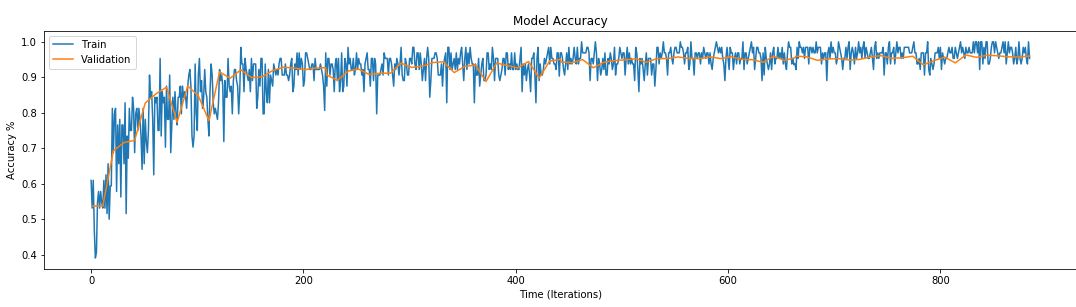
\includegraphics[width=.95\linewidth]{cnn_acc.png}
    \caption{The accuracy for the pure CNN network}
\end{figure}

\subsection{CNN+RNN Hybrid}
This architecture was significantly harder to get working because it was something I was unfamiliar with.
For this model, the input was instead the textual output of \texttt{tcpdump} for the pcap.
This was necessary because there is no easy way to separate a pcap file into individual packets.
The general idea was to use a CNN on each packet (a.k.a. a line of tcpdump output) then feed the outputs of the CNNs into an RNN to handle the sequential aspect of the file.

One difficulty I ran into was the necessity of padding.
I expected to pad along lines of output for the CNN, but did not realize I'd also need to pad out the columns. Even though columns were going through an RNN, the batching process required uniform data.

This model had only \texttt{22,272} parameters. 
This is significantly lower than the previous model, but is mostly due to the use of an RNN.
The architecture consisted of two \texttt{Conv2d} layers followed by an \texttt{LSTM} layer.
There was no particular reason an LSTM was used, other than I was able to find slightly more documentation and support for it.

Like the pure CNN approach, this model achieved $\sim\%90$ accuracy. 
This was a bit disappointing as I had hoped the more complex model would be better.
One suspicion I had was that the first dataset simply didn't have enough data.
However, I did not see any improvement from the second dataset which was five times larger.
It also took significantly longer, at over 2 hours to train, compared to around 30 minutes for the CNN network with dataset 1.

One interesting result of this section is that I had a bug in the first convolution layer giving it a kernel of \texttt{3x3}.
This was unintended since I wanted the convolution to look at only one packet (a.k.a. one line) at a time.
Fixing the kernel to be \texttt{1x3} actual saw slightly worse and less consistent accuracy.

\begin{figure}[H]
    \centering
    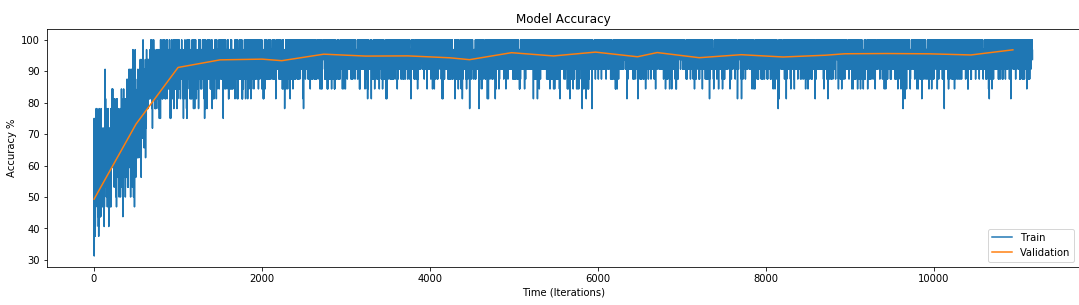
\includegraphics[width=.95\linewidth]{cnn_rnn_acc.png}
    \caption{The accuracy for the RNN+CNN network (with \texttt{3x3} kernel)}
\end{figure}

\subsection{Optimizing Input on Trained Model}
In an attempt to better understand how the models were working, I tried optimizing an input through a trained model to see what the output was.
My hope was that I could create something resembling the pcap data I had created.
I also hoped to see difference in how it generated output for \texttt{web} and \texttt{doh}.

This experimentation was done by generating a tensor of the appropriate size, zeroed out.
The tensor was used by the optimizer and then continually passed into the model.
Loss was calculated by comparing the model's output on the tensor to the desired output.
The tensor was changed by the optimizer using this loss.

Sadly, I saw very little results.
Testing on both the pure CNN network and the CNN+RNN network, I could see the loss get very close to zero.
However, printing out the modified input tensor revealed that it had barely changed at all.
The majority of the tensor was still zeroes with a few values moving up to 1 or 2.
The maximum possible value was 255 in the CNN model (maximum value of one byte) and 100 in the CNN+RNN model (number of printable characters).

Overall, I can't speak too much to these results.
I hypothesize that this is hinting that the network learns very little about classification.
In the CNN+RNN case, I optimized a batch of 1 \texttt{web} and 1 \texttt{doh} input.
Loss got very close to zero, but when running the generated tensors through the model, both were identified as \texttt{web}.

It is also very possible I made some mistakes in this section, but I'm not familiar enough with the process to say where these could be.

\section{Conclusion}
Overall, I feel the architecture could be significantly better, but I am not sure how to improve it.
The accuracy of $\sim\%90$ isn't very impressive considering always guessing \texttt{web} would earn $\sim\%50$ accuracy.

I also had hoped to better understand the reasoning behind the model's choices, but I was unable to successfully do that.
The attempt at generating optimized inputs did not work very well.
I also spent some time trying to print layers of the CNN network as images, but it was unrealistic since the activations were around 1 x 10k.

Despite my somewhat poor results, my model was not a complete failure.
It was able to learn some patterns, although I am not sure what they were.
This is promising for detection of DoH.
Someone with more experience would likely be able to create a better model.
I also purposely limited the data I had to be anonymized and capturing a single query. 
If someone had access to a more complete dataset that showed sequential queries, they may be more successful at identifying patterns.


\subsection{Time Log}
The below table reflects the time spent on this project. I stopped slightly early at 29 hours because I wasn't sure what else could be done. 
I also had the constraint of attending a research conference the last week of school, meaning I needed to finish this project early.
\smallskip

\begin{figure}[H]
    \centering
    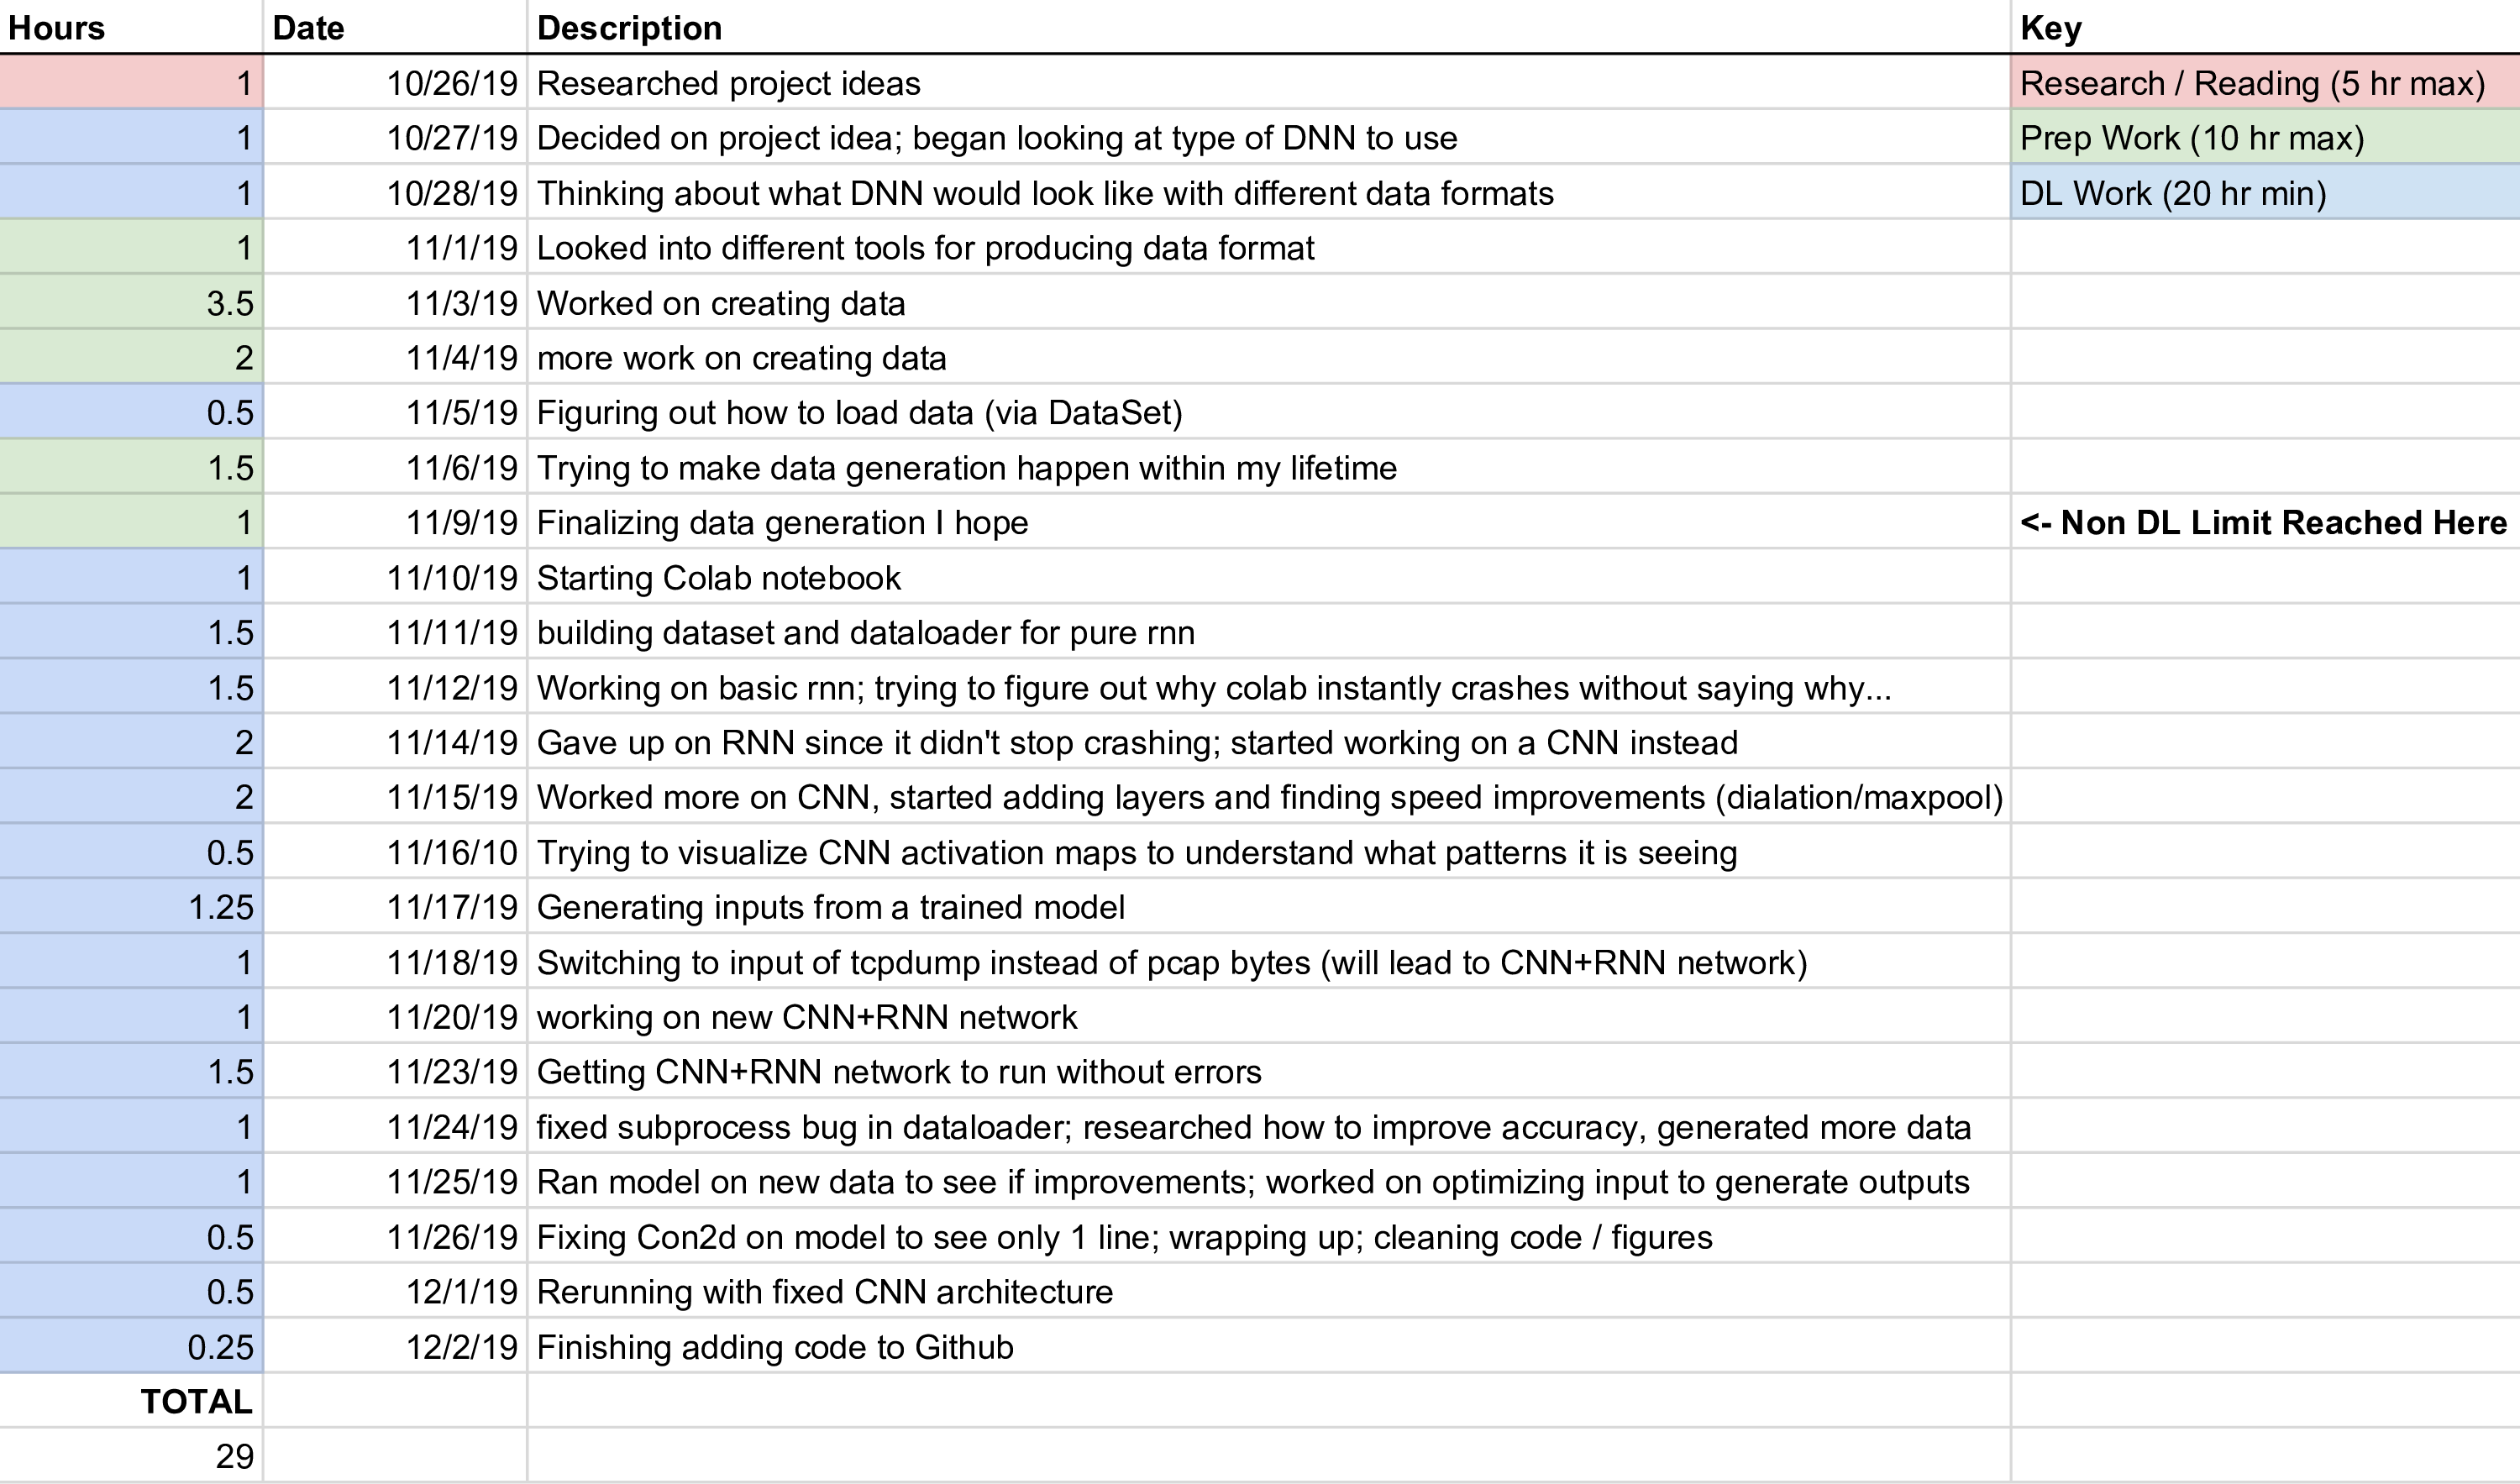
\includegraphics[width=.95\linewidth]{log.png}
\end{figure}

\subsection{Source Code}
All code and data is available at \url{https://github.com/jacobgb24/doh_detection}.\\
Data can be downloaded from the releases section of Github.


\end{document}
